\documentclass[11pt]{article}

\usepackage{geometry}
\usepackage{subcaption} 
\geometry{letterpaper}

\usepackage{doc}
\usepackage{cite}
\usepackage[margin=1cm]{caption}

\usepackage{url}

\usepackage{graphicx}
\usepackage{epstopdf}
\DeclareGraphicsRule{.tif}{png}{.png}{`convert #1 `dirname #1`/`basename #1 .tif`.png}

\title{Dream Design}
\author{Trixie Roque}
\date{11/24/2015}

\begin{document}
\maketitle

\begin{abstract}
The purpose of this paper is to design a new user interface for the Instagram application by integrating timeline options similar to the ones employed by Facebook, as well as allowing the users more freedom in editing their posts. Implementing these features would require integrating other APIs, such as Google Maps, for its ability to create a travel history for the user, and Snapchat, for its ability to grant users the option to doodle on their captured photos. The goal of the interface is to present the user with the power to map out a story based on their travel destination posts. The five usability metrics that are involved, therefore, in the creation of this design idea are learnability, efficiency, and satisfaction.
\end{abstract}

\pagebreak
\tableofcontents

\pagebreak

\section{Introduction}
\label{Introduction}
   \indent 
    \indent Social media applications have become a common tool in our society, especially to millennials. The ability to connect with both friends and strangers alike through the submission of "posts" onto the internet has become so widespread that it is rare to find a person that does not own at least one social media account. Social media has been a gateway for people to communicate by sending clever quips, funny memes, and/or embarrassingly hilarious gifs or videos, among other things. Some people can even say that their hobbies involve sifting through countless blogs, tweets, videos, etc. of internet denizens. Because these social media applications provide us with the capability to peek through the various adventures in other people's lives, we have become incredibly immersed in them. However, even with the continuous appearance of these applications that aim to grab our everyday attention, design improvements are always necessary to cater to the growing number of social media consumers. \\ \\
     \indent In addition to these applications, touchscreen devices have also become a norm. The iPhone, for example, though invented only 8 years ago, has quickly become a popular mobile device for the masses. Phones, in general, have actually evolved into a multi-purpose tool in our everyday lives. Utilizing touch-capable mobile handheld devices as its main system might have even caused the boom in the usage of social media applications. \\ \\
     \indent In this paper, I will focus on a specific social media, one that is mainly used to post pictures for other people to see, called Instagram, focusing on the application that is downloaded through a mobile touch-enabled phone.
     
     
\section{System Description}
\label{System Description}
   \indent 
   \indent Although there is also a desktop client for Instagram, called Webstagram, the main focus of this paper is to address the designs in the mobile application. There is no question that Instagram would be used more frequently through a phone its main appealing quality is its capability to quickly post snapshots in a matter of seconds. A user can easily choose an already existing picture in their camera roll and tap on a few buttons and their pictures can be viewed by their followers. Additionally, users have the option of taking a picture from within the application so that they do not have to switch between it and the built-in camera application in their device. In addition to the picture, the user is also given an option to write a quick description about the image. \\ \\
   \indent The current design of Instagram appears to be already simplistic, which makes it very intuitive to new users. In the interface, users can scroll through their "news" feed, which contains recent posts of users they follow, or they can take a picture themselves and post it on their feed. Figure 1a shows some available tools for the user after they had just taken a picture. Additionally, the user can also "tag" the location where they took that photo. Figure 1b gives a map of the area where a photo was taken and marks those significant places with the corresponding pictures. For example, in Figure 1b, three pictures were taken near Chiu Tam Path, Hong Kong. The availability of this kind of map gives the user a more visual overview of the places they had visited in the past. 
   \indent These figures present a way to further improve upon the interface of Instagram. Although there are various photo editing tools in Instagram, it lacks the ability to manually draw on the pictures directly. Using Snapchat, another popular social media where the user sends pictures to others, as an example, it is evident that consumers would find the freedom to doodle on the pictures to be satisfying. Moreover, with respect to the map functionality seen in Figure 1b, there is a potential to actually create a more GPS-like feature so that users can trace back exactly which places the user visited first.
      
\begin{figure}[ht]
\centering
\begin{subfigure}[b]{.5\textwidth}
   \centering
    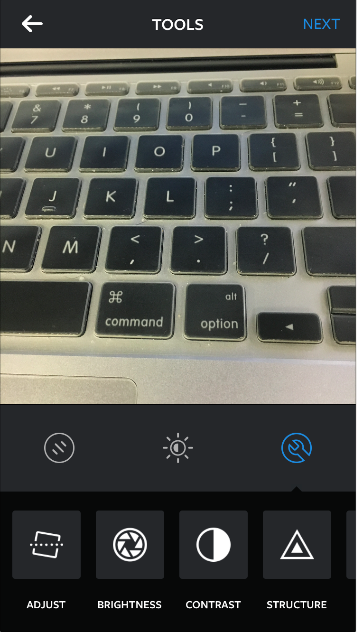
\includegraphics[height=\textwidth]{images/instagram_tools.png}
    \caption{Some tools that exist in Instagram's interface include brightness adjustments.}
    \label{tools}
\end{subfigure}%
~~~~~~~
\begin{subfigure}[b]{.5\textwidth}
    \centering
    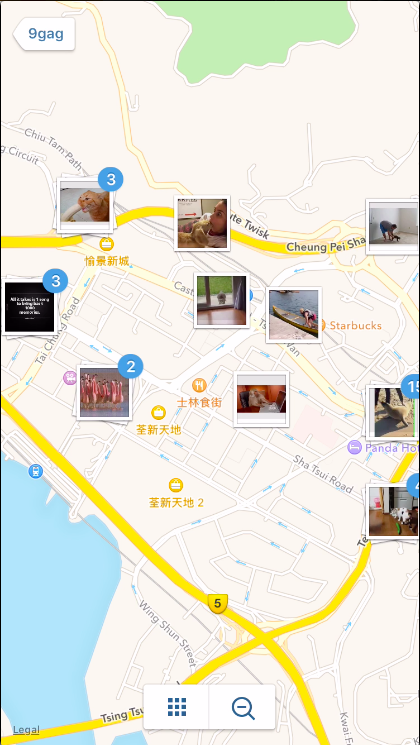
\includegraphics[height=\textwidth]{images/maps_with_pictures.png}
    \caption{Instagram allows users to group pictures together based on where they were taken.}
    \label{instagram_pictures}
\end{subfigure}
\caption{Some features that are available in the Instagram interface}
\end{figure}

\section{Top-Level Design}
\label{Top-Level Design}
   \indent 
   \indent In order to accommodate the additional features that will be involved, the integration of various other APIs into Instagram is a must since its own API lack these functionalities. From looking at Figure 1b, it would seem that Instagram is already utilizing the Google Maps API, though I would argue that it isn't being used to its fullest potential. 1b is only using the pictures as "pins" to mark special places, but the Google Maps API is capable of much more. One such feature is the ability to create a timeline history of visited places, which, when implemented, would grant the users the option to view their past journeys. The overall design for that particular aspect of Instagram would be incorporating the two APIs such that a user can view their maps in a GPS-like fashion. That is, the map would contain lines that visually connect two pictures (but would actually be linking two locations together) so that the Instagrammer can follow where they have been to or locate the area where they tend to explore. Figure 2 depicts what a certain user's "footprint" might look like, albeit they would be given an option to separate different paths, similar to how one can choose a path from a 2 or 3 different options when using a GPS device. \\
   
\begin{figure}[ht]
\centering
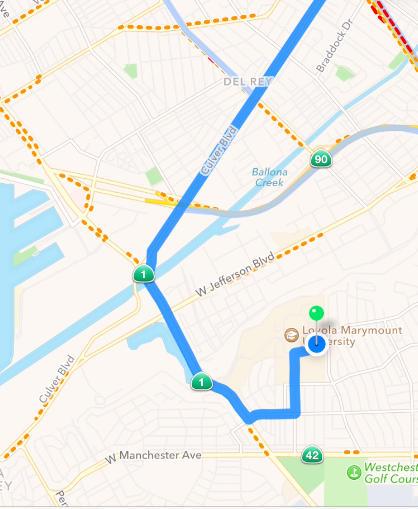
\includegraphics[width=3in]{images/gps.png}
\caption{Similar to a GPS path, the blue line would heuristically map out the path that the user took based on their posts.}
\label{travel_history}
\end{figure}

   \indent In Figure 2, the green dot will be replaced by a post with a specified location when the feature is implemented into Instagram. Similar to the Google Maps feature to redirect paths, the user will also be given an option to drag the path in order to manually draw the routes they have traversed. Of course, this figure is showing only one case for one specific path that the user took to get from one place to another. For cases where the user took a more significant number of pictures and posted them on his/her feed, Figure 3 demonstrates what the map could look like. \\

\begin{figure}[ht]
\centering
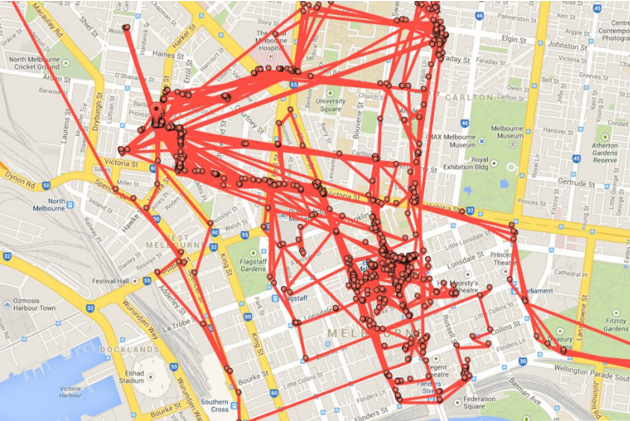
\includegraphics[width=5in]{images/google_maps_tracking.png}
\caption{Google Maps tracks users' travel history}
\label{google_tracking}
\end{figure}

   \indent In the figure above, the circles, which indicate places of interest, would also be replaced by the pictures that the user posted on their feed (similar to what is seen in Figure 1b). Note that the user can still zoom in and out of the map in order to see the map more closely or in less detail. If viewed in lesser detail such that the pictures overlap, then those would just be grouped together. Again, this is similar to Figure 1b, where there is a number on the upper-right corner of a given picture to indicate how many are overlapping; for instances where this happen, the posts would be grouped chronologically such that the most recent post is what is seen.\\ \\
   \indent Additional features that would improve the users' experience with this feature is to actually show the exact date, time, and address of their posts. By doing this, the users can log exactly where they were at what times, if they wish. The user will also be given an option to delete such information from their "adventure". Figure 4 shows what this feature would look like when implemented. \\ \\
   
\pagebreak

\begin{figure}[ht]
\centering
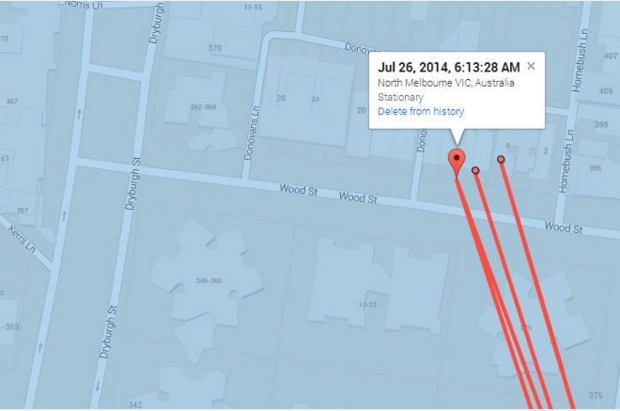
\includegraphics[width=5in]{images/google_maps_tracking_with_info.png}
\caption{The new interface would give the options to view information about the event or delete it.}
\label{google_tracking}
\end{figure}

   \indent For the feature that employs Snapchat's photo-drawing capabilities, one simple addition to the interface is all that is needed. Figure 5 shows the layout for the new design. Here, the layout will keep the original design of the screen after a photo has been taken (as seen in Figure 1a) but there would be an additional vertical color gradient slider at the upper right hand corner similar to the one used by Snapchat. In order to avoid the problem of accidentally tapping the gradient slider, this feature can be accessed through the Tools section and will only appear when it is enabled. The user can flip through the various other tools by using a flicking motion. 
      
\begin{figure}[ht]
\centering
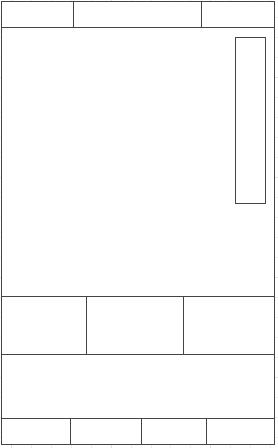
\includegraphics[width=2in]{images/wireframe.png}
\caption{The vertical slider located in the upper-right hand corner of the screen will allow the user to choose which font color they wish to use.}
\label{wireframe}
\end{figure}

\pagebreak
   
\section{Usage Scenarios}
\label{Usage Scenarios}
   \indent
   \indent The main purpose of the new features is to improve the user experience for the Instagram mobile application. As with the original mental model for Instagram, the user can still post any pictures of their choosing onto their respective news feeds. However, with the addition of the map-like feature, users can easily log the places they have been to, which is similar to an online picture diary. A possible scenario to this would be when the user is studying abroad and would like to record their adventures. For college students especially, having the opportunity to explore another country with their peers and still continue their studies is an experience worth cherishing. By posting to Instagram and marking when and where exactly they were during their stay abroad, they can revisit those memories in the future or even view which areas they haven't explored yet. \\ \\
   \indent For the added drawing capabilities, making the pictures act more like canvases allows the user to more freely express their ideas. Practically any scenario that involves taking a picture and providing a caption would apply to this feature. For specificity's sake, we can say that a couple of stressed college students want to release their feelings of tension by trying to prank each other. They can do so by taking an innocent-looking picture of each other, but manually inserting their creativity into the picture using their fingertips. Figure 6 shows what a creative, witty person might come up with when allowed the option to draw on a photograph.

\begin{figure}[ht]
\centering
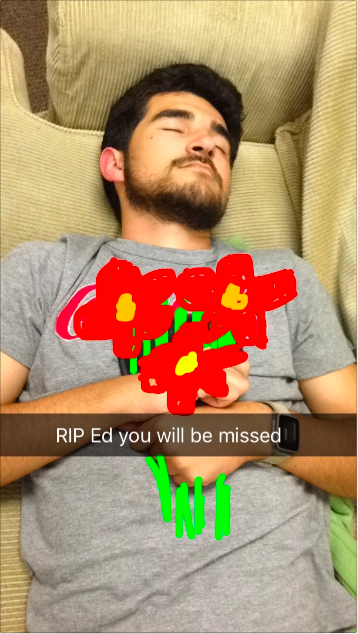
\includegraphics[height=4in]{images/rip_ed.png}
\caption{An example of doodling on a picture. The flowers were hand-drawn directly on the picture. Note: The person in the picture has granted me permission to use this picture.}
\label{ed}
\end{figure}

\pagebreak

\section{Rationale}
   \indent
   \indent The driving force for the new interaction design to Instagram is to grant users with a more enjoyable experience with the application. As with mobile applications, there has to be a hook for people to continue using the product. The reason why developers continuously provide updates to their applications is so that the users do not become bored of the same old features. Even applications that possess a large number of users like Instagram would eventually lose consumers if there is nothing new that it can offer. \\ \\
   \indent The creation of these potential design implementations would not only provide a potentially better way to document the lives of Instagram users, but would also take advantage of the touch-screen's capabilities without destroying the original mental model concept that its creators imagined. In fact, since Instagram is mainly used for documenting experiences via pictures, adding these new designs would actually enhance those already existing functionalities.The new features would simply act as extensions of these existing tools.  Additionally, since the users would be making more direct manipulation of objects when utilizing the various options within Instagram, they would actually be using a feature that is unique to touch devices. 
         
\section{Usability Metric ``Forecast''}
   \indent 
   \indent Since the new design would integrate features that other APIs present, the usability metrics would have to be discussed in order to keep in mind how the user would interact with the interface. As discussed in class. If the designs are successfully implemented and tested, given enough time, money, and manpower, the strongest metrics, as discussed in class, would be satisfaction and learnability. In contrast, the metrics that might suffer from the implementation would be the error metric, and possibly the memorability metric.\\ \\
   \indent Because the purpose of the interface is to grant more features for users when they create their posts, consumer satisfaction is a necessary metric to fulfill. The ability to generate a path containing the places that a person has visited would allow the users to both keep a record of their journeys, as well as revisit their old memories of those journeys through a map-like interface. With respect to doodling using the touch interface, it would be more satisfactory to the user to be given more options when using an application. Additionally, with regards to learnability, since the new features are actually extensions of the existing features, previous users would actually already possess the necessarily skills to navigate through the additional features. Because of this, it would be extremely easy for them to learn how to use the new features; this is especially true with regards to the doodling feature.\\ \\
   \indent Nonetheless, there is a backside to the added features. Because of more options, thus more buttons, the likelihood that the user encounters errors would definitely increase since the user would have more options when tapping. Since some phones might differ in sensitivity when the users tap on items, the users can easily select an option they didn't intend. Especially with the map-like feature, manual dragging of a route might actually prove difficult to the user. Users might actually find it more troublesome to drag a line around than letting the program predict the route that was taken. With the drawing feature, the error that might arise would be when the user tries to draw in the exact space where the slider exists. In order to mitigate the errors that might arise for the doodles, the slider can be enabled or disabled, as briefly described in the above sections.\\ \\

\clearpage

\bibliographystyle{plain}
\end{document}

\end{document}